\documentclass[12pt,a4paper]{article}

% Packages
\usepackage{amsmath}
\usepackage{amsfonts}
\usepackage{amssymb}
\usepackage{graphicx}
\usepackage[margin=1in]{geometry}
\usepackage{enumitem}
\usepackage[hidelinks]{hyperref}
\usepackage{xcolor}

% Title
\title{Homework Report for Computer Vision}
\author{Yu Xiang, Luo}
\date{\today}

\begin{document}

\maketitle

\[
	\href{https://github.com/YuXiangLo/Computer-Vision}{\text{\textcolor{blue}{You can check this github for more information}}}
\]

\begin{enumerate}[label=(\alph*)]
	\item Downsampling Lena to $64 \times 64$:\\
		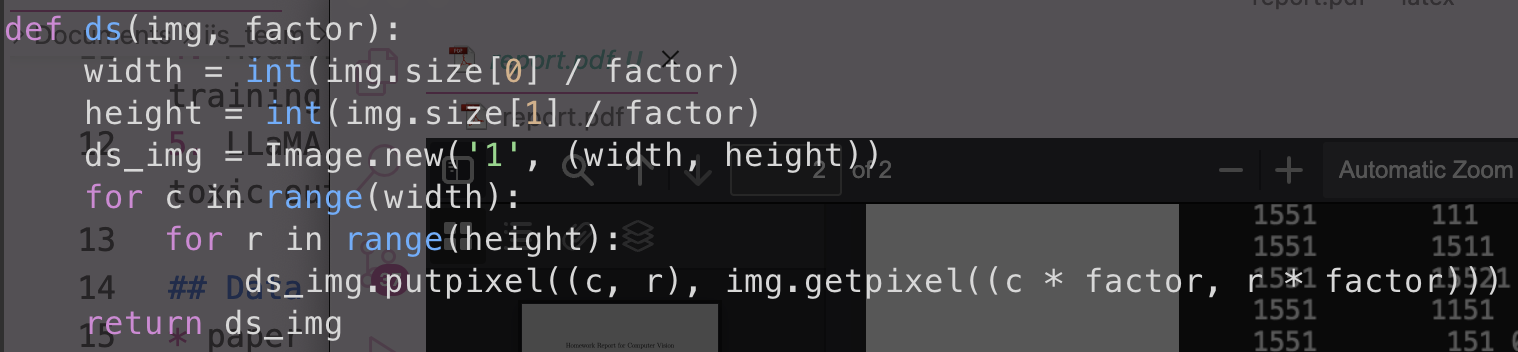
\includegraphics[width=0.9\textwidth]{./img/ds_code.png}\\
		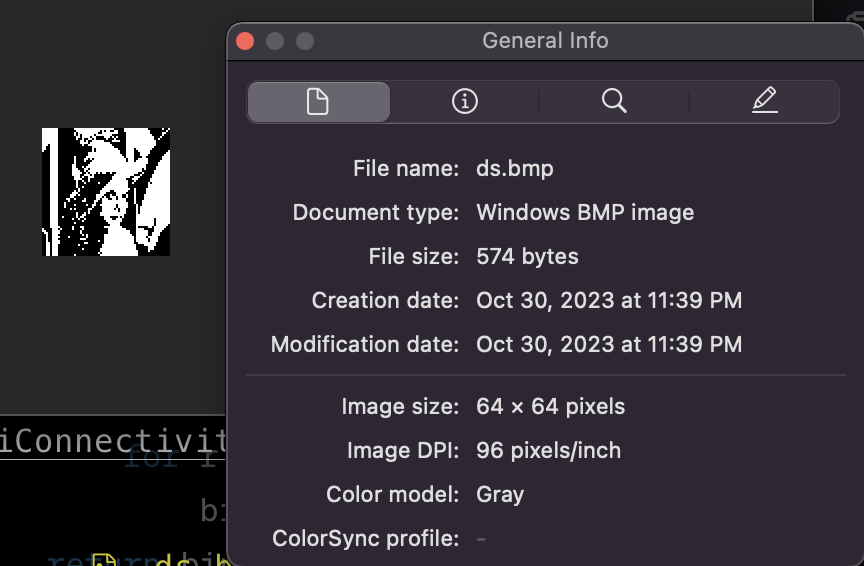
\includegraphics[width=0.9\textwidth]{./img/ds.png}\\
	\item yokoi:\\
		In this code, we need to record the neighbor pixel, then we check h function to see if two neighbors are the same, or only just one. In the end, we use f to aggregate the infomation.\\
		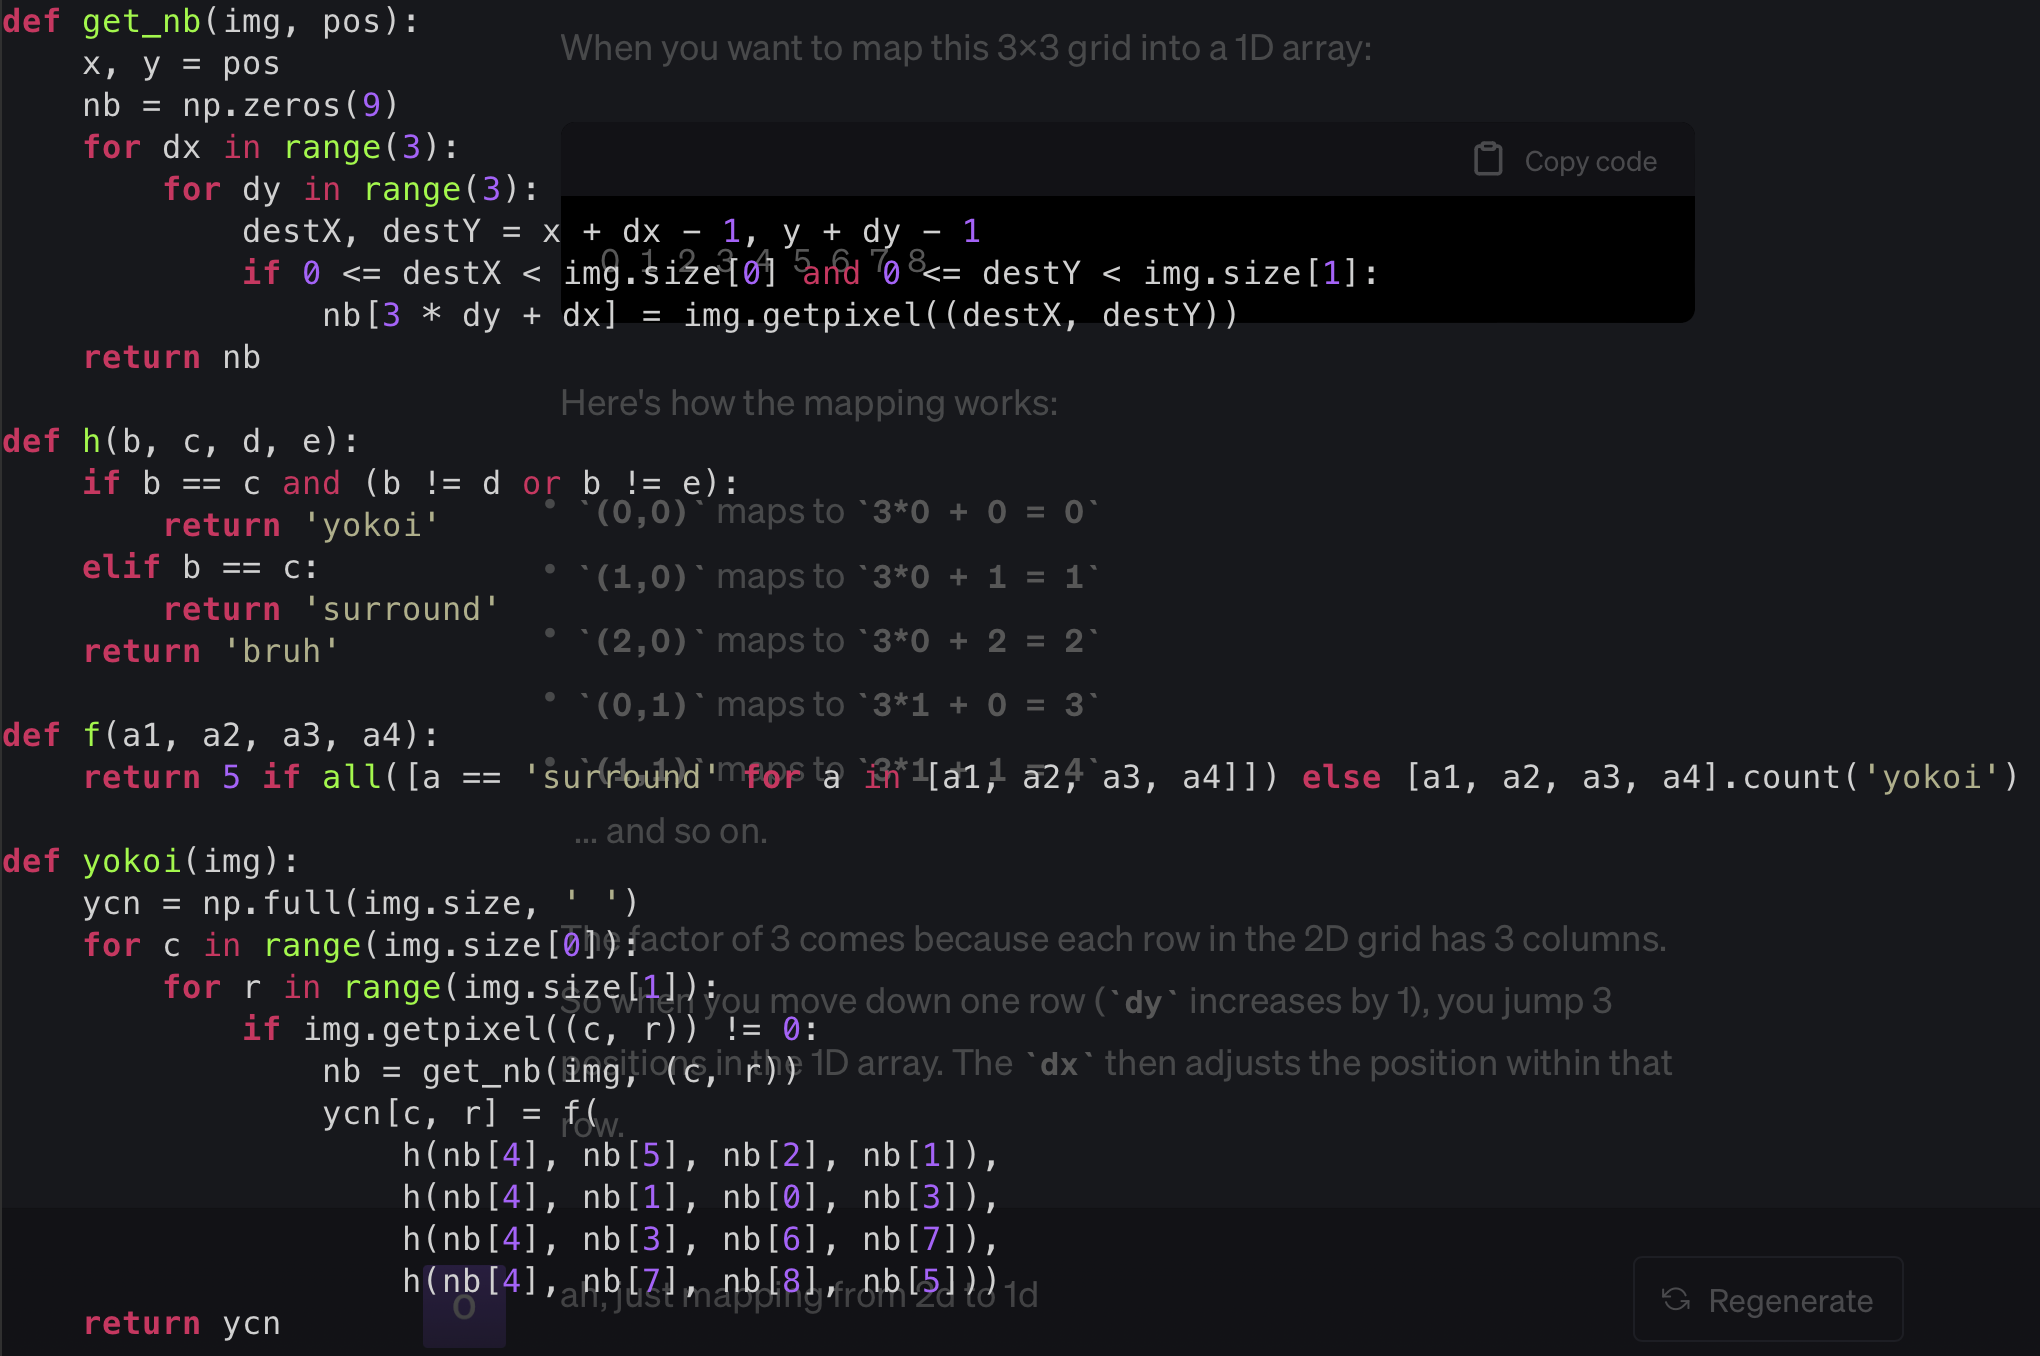
\includegraphics[width=0.9\textwidth]{./img/yokoi_code.png}\\
		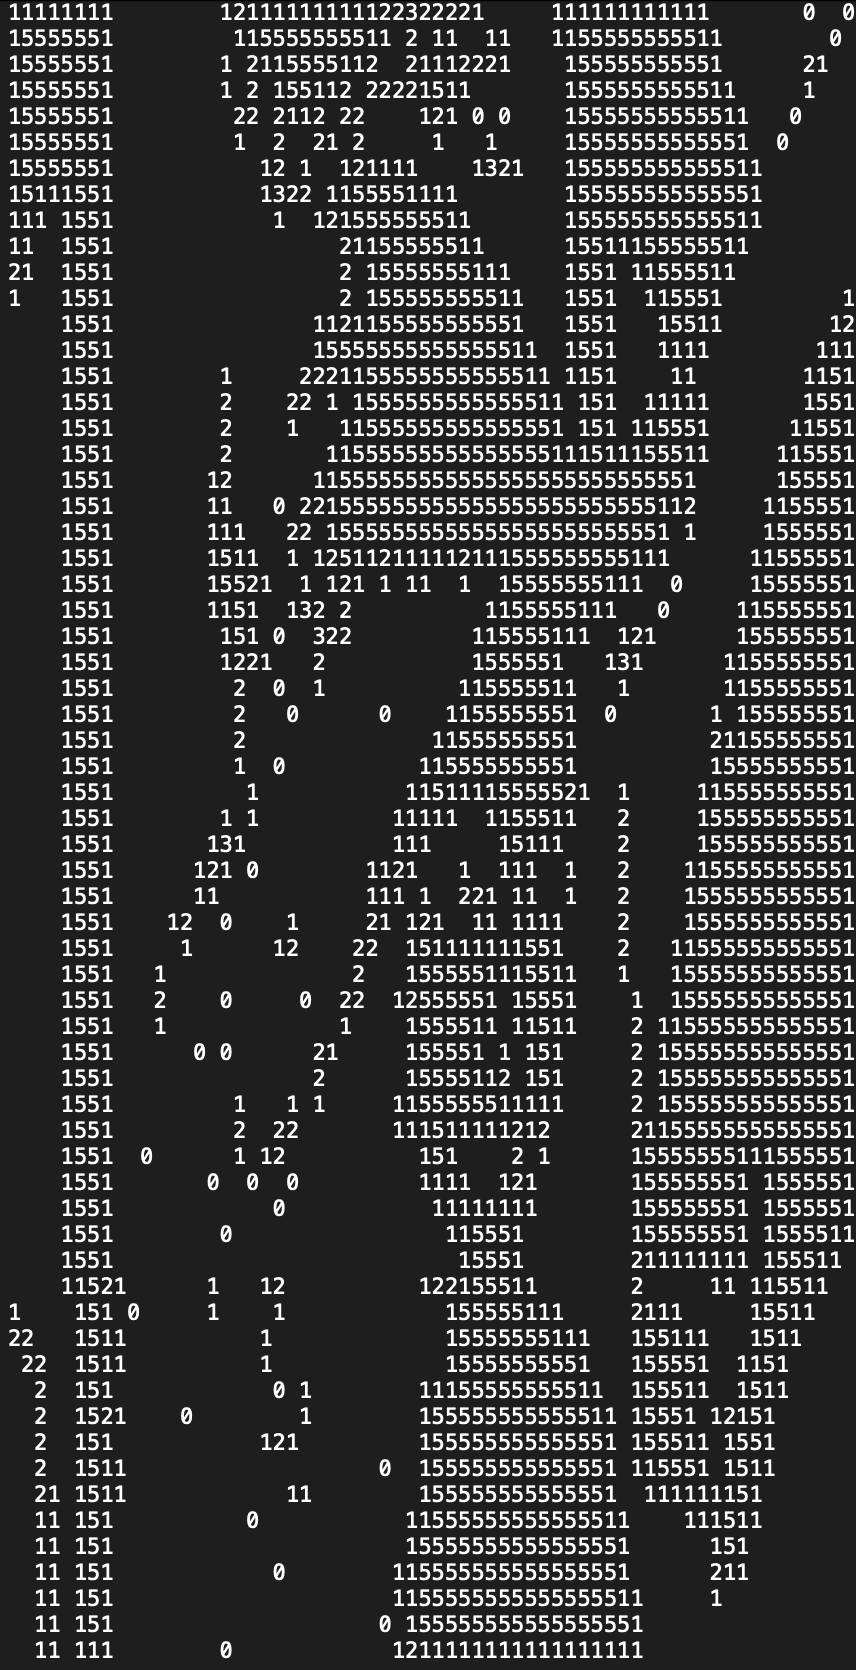
\includegraphics[width=0.9\textwidth]{./img/yokoi.png}\\
\end{enumerate}



\end{document}
